% Options for packages loaded elsewhere
\PassOptionsToPackage{unicode}{hyperref}
\PassOptionsToPackage{hyphens}{url}
\PassOptionsToPackage{dvipsnames,svgnames,x11names}{xcolor}
%
\documentclass[
  12pt,
  letterpaper,
]{scrreprt}

\usepackage{amsmath,amssymb}
\usepackage{setspace}
\usepackage{iftex}
\ifPDFTeX
  \usepackage[T1]{fontenc}
  \usepackage[utf8]{inputenc}
  \usepackage{textcomp} % provide euro and other symbols
\else % if luatex or xetex
  \usepackage{unicode-math}
  \defaultfontfeatures{Scale=MatchLowercase}
  \defaultfontfeatures[\rmfamily]{Ligatures=TeX,Scale=1}
\fi
\usepackage{lmodern}
\ifPDFTeX\else  
    % xetex/luatex font selection
  \setmainfont[]{Times New Roman}
  \setsansfont[]{Arial}
  \setmonofont[]{Courier New}
\fi
% Use upquote if available, for straight quotes in verbatim environments
\IfFileExists{upquote.sty}{\usepackage{upquote}}{}
\IfFileExists{microtype.sty}{% use microtype if available
  \usepackage[]{microtype}
  \UseMicrotypeSet[protrusion]{basicmath} % disable protrusion for tt fonts
}{}
\usepackage{xcolor}
\usepackage[inner=2.54cm,outer=2.54cm,top=2.54cm,bottom=2.54cm,headsep=22pt,headheight=11pt,footskip=33pt,ignorehead,ignorefoot,heightrounded]{geometry}
\setlength{\emergencystretch}{3em} % prevent overfull lines
\setcounter{secnumdepth}{5}
% Make \paragraph and \subparagraph free-standing
\ifx\paragraph\undefined\else
  \let\oldparagraph\paragraph
  \renewcommand{\paragraph}[1]{\oldparagraph{#1}\mbox{}}
\fi
\ifx\subparagraph\undefined\else
  \let\oldsubparagraph\subparagraph
  \renewcommand{\subparagraph}[1]{\oldsubparagraph{#1}\mbox{}}
\fi


\providecommand{\tightlist}{%
  \setlength{\itemsep}{0pt}\setlength{\parskip}{0pt}}\usepackage{longtable,booktabs,array}
\usepackage{calc} % for calculating minipage widths
% Correct order of tables after \paragraph or \subparagraph
\usepackage{etoolbox}
\makeatletter
\patchcmd\longtable{\par}{\if@noskipsec\mbox{}\fi\par}{}{}
\makeatother
% Allow footnotes in longtable head/foot
\IfFileExists{footnotehyper.sty}{\usepackage{footnotehyper}}{\usepackage{footnote}}
\makesavenoteenv{longtable}
\usepackage{graphicx}
\makeatletter
\def\maxwidth{\ifdim\Gin@nat@width>\linewidth\linewidth\else\Gin@nat@width\fi}
\def\maxheight{\ifdim\Gin@nat@height>\textheight\textheight\else\Gin@nat@height\fi}
\makeatother
% Scale images if necessary, so that they will not overflow the page
% margins by default, and it is still possible to overwrite the defaults
% using explicit options in \includegraphics[width, height, ...]{}
\setkeys{Gin}{width=\maxwidth,height=\maxheight,keepaspectratio}
% Set default figure placement to htbp
\makeatletter
\def\fps@figure{htbp}
\makeatother
% definitions for citeproc citations
\NewDocumentCommand\citeproctext{}{}
\NewDocumentCommand\citeproc{mm}{%
  \begingroup\def\citeproctext{#2}\cite{#1}\endgroup}
\makeatletter
 % allow citations to break across lines
 \let\@cite@ofmt\@firstofone
 % avoid brackets around text for \cite:
 \def\@biblabel#1{}
 \def\@cite#1#2{{#1\if@tempswa , #2\fi}}
\makeatother
\newlength{\cslhangindent}
\setlength{\cslhangindent}{1.5em}
\newlength{\csllabelwidth}
\setlength{\csllabelwidth}{3em}
\newenvironment{CSLReferences}[2] % #1 hanging-indent, #2 entry-spacing
 {\begin{list}{}{%
  \setlength{\itemindent}{0pt}
  \setlength{\leftmargin}{0pt}
  \setlength{\parsep}{0pt}
  % turn on hanging indent if param 1 is 1
  \ifodd #1
   \setlength{\leftmargin}{\cslhangindent}
   \setlength{\itemindent}{-1\cslhangindent}
  \fi
  % set entry spacing
  \setlength{\itemsep}{#2\baselineskip}}}
 {\end{list}}
\usepackage{calc}
\newcommand{\CSLBlock}[1]{\hfill\break\parbox[t]{\linewidth}{\strut\ignorespaces#1\strut}}
\newcommand{\CSLLeftMargin}[1]{\parbox[t]{\csllabelwidth}{\strut#1\strut}}
\newcommand{\CSLRightInline}[1]{\parbox[t]{\linewidth - \csllabelwidth}{\strut#1\strut}}
\newcommand{\CSLIndent}[1]{\hspace{\cslhangindent}#1}

\addtokomafont{disposition}{\rmfamily}
\KOMAoptions{chapterprefix=false,appendixprefix=true} %% chapterprefix=true para que aparezca como capitulo 1 o =false para que solo aparezca el numero romano
\KOMAoptions{headings=small}
\raggedright
\setkomafont{pageheadfoot}{\normalfont\normalcolor\footnotesize}
\setkomafont{pagenumber}{\normalfont\normalcolor\footnotesize}
\renewcommand{\thechapter}{\Roman{chapter}}
\renewcommand{\thesection}{\arabic{chapter}.\arabic{section}}
\renewcommand{\thefigure}{\arabic{figure}}
\renewcommand{\thetable}{\arabic{table}}
\renewcommand{\theequation}{\arabic{equation}}
\usepackage{ragged2e}
\justifying
\makeatletter
\@ifpackageloaded{bookmark}{}{\usepackage{bookmark}}
\makeatother
\makeatletter
\@ifpackageloaded{caption}{}{\usepackage{caption}}
\AtBeginDocument{%
\ifdefined\contentsname
  \renewcommand*\contentsname{Tabla de contenidos}
\else
  \newcommand\contentsname{Tabla de contenidos}
\fi
\ifdefined\listfigurename
  \renewcommand*\listfigurename{Índice de figuras}
\else
  \newcommand\listfigurename{Índice de figuras}
\fi
\ifdefined\listtablename
  \renewcommand*\listtablename{Listado de Tablas}
\else
  \newcommand\listtablename{Listado de Tablas}
\fi
\ifdefined\figurename
  \renewcommand*\figurename{Figura}
\else
  \newcommand\figurename{Figura}
\fi
\ifdefined\tablename
  \renewcommand*\tablename{Tabla}
\else
  \newcommand\tablename{Tabla}
\fi
}
\@ifpackageloaded{float}{}{\usepackage{float}}
\floatstyle{ruled}
\@ifundefined{c@chapter}{\newfloat{codelisting}{h}{lop}}{\newfloat{codelisting}{h}{lop}[chapter]}
\floatname{codelisting}{Listado}
\newcommand*\listoflistings{\listof{codelisting}{Listado de Listados}}
\captionsetup{labelsep=colon}
\makeatother
\makeatletter
\makeatother
\makeatletter
\@ifpackageloaded{caption}{}{\usepackage{caption}}
\@ifpackageloaded{subcaption}{}{\usepackage{subcaption}}
\makeatother
\ifLuaTeX
\usepackage[bidi=basic]{babel}
\else
\usepackage[bidi=default]{babel}
\fi
\babelprovide[main,import]{spanish}
\ifPDFTeX
\else
\babelfont{rm}[]{Times New Roman}
\fi
% get rid of language-specific shorthands (see #6817):
\let\LanguageShortHands\languageshorthands
\def\languageshorthands#1{}
\ifLuaTeX
  \usepackage{selnolig}  % disable illegal ligatures
\fi
\usepackage{bookmark}

\IfFileExists{xurl.sty}{\usepackage{xurl}}{} % add URL line breaks if available
\urlstyle{same} % disable monospaced font for URLs
\hypersetup{
  pdftitle={Unidad de Estadística - UNSAAC},
  pdfauthor={Oscar Chullo Puclla; Betty Alegre Ramos},
  pdflang={es},
  colorlinks=true,
  linkcolor={blue},
  filecolor={Maroon},
  citecolor={Blue},
  urlcolor={Blue},
  pdfcreator={LaTeX via pandoc}}

\title{Unidad de Estadística - UNSAAC}
\author{Oscar Chullo Puclla \and Betty Alegre Ramos}
\date{2024}

\begin{document}
\pagenumbering{roman} %%numeracion en numeros romanos para la primera parte
%% justo hasta antes de indice
\thispagestyle{empty}
\hspace{0.075\textwidth} 
\begin{minipage}[b][\textheight][s]{0.85\textwidth}

%% Formalidad, encabezado nombrev de: U,Facultad,etc
\centering
\textbf{\large{Universidad Nacional de San Antonio Abad del Cusco}} \\
\textbf{\large{Facultad de ciencias físicas, químicas y matemáticas}} \\
\textbf{\large{Escuela profesional de matemáticas y estadística}} \\
\textbf{\large{}} \\ %% subtitle es para nominación del año
\vspace{1\baselineskip}

%% Logo central

\includegraphics[width=6cm]{imagen/unsaac.png}
\vspace{1\baselineskip}

% Parte tesis encuadrada
\Large{\textbf{INFORME DE PRÁCTICAS PRE-PROFESIONALES:}} \\
\hrulefill \\
{\Large\bfseries{Unidad de Estadística - UNSAAC}} \\
\hrulefill 

% Abstract


\large{
\flushleft \hspace{6cm}
\textbf{JEFE DE LA UNIDAD DE} \\\hspace{6cm}
\textbf{ESTADÍSTICA:} \\
\hspace{6cm} Econ. Carlos Huamán Aguilar \\ 
\smallskip
\hspace{6cm} \textbf{PRESENTADO POR:} \\ \hspace{6cm}
 {\large{Oscar Chullo Puclla}}
\\
\smallskip
\hspace{6cm} \textbf{DOCENTE:} \\ \hspace{6cm}
%
{\large{Betty Alegre Ramos}}%

}

\vfill

\centering
\Large{CUSCO - PERÚ} \\
\Large{2024}
\vspace{0.1\textheight} 
\end{minipage}

%%% Colocar capitulo y pagina sobre el índice
\addtocontents{toc}{\hspace{-0.1mm} \textbf{Capítulos}}
\addtocontents{toc}{\hfill \textbf{Página} \par}
\addtocontents{toc}{\vspace{-2mm} \hspace{-7.5mm} \hrule \par}

%%% Editar dedicatoria

\pagebreak %% no quitar porque se juntara todo

%% Editar agradecimiento

\setlength{\parindent}{1.5em}

\renewcommand*\contentsname{Índice general}
{
\hypersetup{linkcolor=}
\setcounter{tocdepth}{2}
\tableofcontents
}
\listoffigures
\setstretch{2}
\bookmarksetup{startatroot}

\chapter{Introducción}\label{introducciuxf3n}

\pagenumbering{arabic}

Las prácticas pre-profesionales nos permiten integrar los conocimientos
y habilidades adquiridas en la formación académica, puesto que estas
constituyen una fase clave en el desarrollo profesional. En este
contexto, se ha tenido la oportunidad de realizar Prácticas
Pre-Profesionales (PPP) en la Universidad Nacional de San Antonio Abad
del Cusco, en particular en la Unidad de Estadística.

Esta oficina se encuentra ubicada en el pabellón del instituto de
idiomas, tercer piso, las prácticas se desarrollaron durante cinco horas
diarias, de 8:00 a.m. a 1:00 p.m. El periodo de tiempo establecido fue
de cuatro meses, se desarrolló diversas actividades durante este periodo
resaltándose los estadísticos para el compendio estadístico 2024, el
costo financiero por alumno 2019-2023 y la organización de bases de
datos

El presente informe ofrece un relato detallado de las funciones
desempeñadas durante el periodo de las prácticas pre-profesionales.

\bookmarksetup{startatroot}

\chapter{Unidad de Estadística}\label{unidad-de-estaduxedstica}

La Unidad de Estadística es una Unidad Orgánica comprendida dentro de la
organización de la Direccion de Sistemas de Informacion, tiene a su
cargo la recopilación, sistematización, análisis y publicación de los
datos estadísticos necesarios para la planificación y programación de
las actividades que desarrolla la universidad, realiza estudios y
diagnósticos sociales, económicos y académicos.(Estadística, 2024)

\section{Funciones}\label{funciones}

\begin{itemize}
\tightlist
\item
  Ejecutar las actividades estadísticas de acuerdo a los requerimientos
  institucionales.
\item
  Capturar, elaborar, revisar, criticar validar y procesar para su
  difusión, las estadísticas a fin de facilitar la gestión y toma de
  decisiones.
\item
  Suministrar datos estadísticos solicitados por las diferentes
  dependencias del Nivel Nacional, Regional, Local e institucional.
\item
  Asesorar a la Alta Dirección en asuntos de manejo de información
  estadística.
\item
  Realizar estudios estadísticos sobre aspectos diversos de la
  problemática universitaria que permita un mejor conocimiento de la
  realidad.
\item
  Elaborar indicadores e índices económicos y sociales para el análisis
  y formulación de políticas institucionales.
\item
  Establecer métodos para el cálculo de tendencias y/o proyecciones
  estadísticas.
\item
  Realizar diagnósticos sociales económicos y académicos de la
  Universidad.
\item
  Publicar anualmente boletines estadísticos, trípticos y otros
  documentos.
\item
  Organizar y administrar el banco de datos estadísticos de la
  institución.
\item
  Velar por la capacitación permanente del personal del Área.
\item
  Elaborar el plan de trabajo anual del Área.
\item
  Coordinar la recopilación, procesamiento de datos estadísticos con las
  diferentes dependencias de la institución.
\end{itemize}

\section{Organización}\label{organizaciuxf3n}

\begin{enumerate}
\def\labelenumi{\arabic{enumi}.}
\tightlist
\item
  \textbf{Órgano de Dirección:} ``Unidad de Estadística''
\end{enumerate}

\begin{itemize}
\tightlist
\item
  \textbf{Órganos de Línea:} ``Unidad de Recopilación, procesamiento y
  análisis estadístico'' y ``Unidad de Estudios socio económicos''
\end{itemize}

\begin{enumerate}
\def\labelenumi{\arabic{enumi}.}
\setcounter{enumi}{1}
\tightlist
\item
  \textbf{Personal del Área:}
\end{enumerate}

\begin{itemize}
\tightlist
\item
  \textbf{Jefe de la Unidad de Estadística:} Econ CARLOS HUAMAN AGUILAR
\item
  \textbf{Teléfono:} 989414939
\item
  \textbf{Anexo:} 1004,
\item
  \textbf{correo electrónico:} estadistica@unsaac.edu.pe
\end{itemize}

\section{Misión}\label{misiuxf3n}

Producir y difundir las estadísticas de la UNSAAC con calidad y
transparencia para la toma de decisiones en materia académica,
administrativa y política institucional.

\section{Visión}\label{visiuxf3n}

Ser reconocida, como la fuente fundamental de las estadísticas de la
UNSAAC por la calidad en sus productos y servicios ofrecidos a los
demandantes.

\bookmarksetup{startatroot}

\chapter{Desarrollo de Prácticas Pre-Profesionales
(PPP)}\label{desarrollo-de-pruxe1cticas-pre-profesionales-ppp}

\section{Setiembre}\label{setiembre}

\subsection{Elaboracion del registro de bachilleres y titulados de la
escuela profesional de Ingeniería Informática y de Sistemas
(1993-2023)}\label{elaboracion-del-registro-de-bachilleres-y-titulados-de-la-escuela-profesional-de-ingenieruxeda-informuxe1tica-y-de-sistemas-1993-2023}

La primera actividad realizada fue la de elaborar un registro completo
de bachilleres y titulados de la E.P. de Ingeniería Informática y de
Sistemas, durante el periodo 1993-2023 bajo solicitud del Director de
escuela correspondiente, se hizo una revision de recursos dentro de la
Unidad de Estadística en los cuales se evidenciaron las siguientes
dificultades: - Falta de Organización en los documentos y la información
de años pasados. - Pérdida de Información de los registros
correspondientes al año 2007, no hubo en libros ni en los CD´s.

Por ello se remitió un registro del periodo 1993-2023 a excepción del
2007.

\subsection{Elaboración de estadísticos de los estudiantes matriculados
del semestre
2024-I}\label{elaboraciuxf3n-de-estaduxedsticos-de-los-estudiantes-matriculados-del-semestre-2024-i}

Se realizo una limpieza de datos en el registro de estudiantes
matriculados correspondientes al semestre 2024-I, puesto que se tenia
error en el registro de sexo (varones registrados como mujeres y
viceversa), e información faltante en los lugares de procedencia, años
de nacimiento y edades, recurriendose al uso de tecnicas de imputación
de datos adquiridos en la formación como estadístico. A continuación se
presentan los resultados obtenidos en grafícos:

\begin{figure}[H]

\caption{Alumnos matriculados según sexo, semestre 2024-I}

{\centering \includegraphics[width=0.7\textwidth,height=\textheight]{imagen/imagen3.png}

}

\end{figure}%%
\begin{figure}[H]

\caption{Alumnos matriculados según facultad, semestre 2024-I}

{\centering \includegraphics[width=0.6\textwidth,height=\textheight]{imagen/imagen5.png}

}

\end{figure}%%
\begin{figure}[H]

\caption{Alumnos matriculados según facultad y sexo, semestre 2024-I}

{\centering \includegraphics{imagen/imagen4.png}

}

\end{figure}%%
\begin{figure}[H]

\caption{Alumnos matriculados según escuelas profesionales, semestre
2024-I}

{\centering \includegraphics{imagen/imagen2.png}

}

\end{figure}%%
\begin{figure}[H]

\caption{Alumnos matriculados por escuelas profesionales y sexo,
semestre 2024-I}

{\centering \includegraphics{imagen/imagen1.png}

}

\end{figure}%%
\begin{figure}[H]

\caption{Alumnos matriculados según región de procedencia, semestre
2024-I}

{\centering \includegraphics[width=0.6\textwidth,height=\textheight]{imagen/imagen6.png}

}

\end{figure}%%
\begin{figure}[H]

\caption{Alumnos matriculados de la región Cusco, semestre 2024-I}

{\centering \includegraphics[width=0.6\textwidth,height=\textheight]{imagen/imagen8.png}

}

\end{figure}%%
\begin{figure}[H]

\caption{Alumnos matriculados de la provincia del Cusco, semestre
2024-I}

{\centering \includegraphics[width=0.6\textwidth,height=\textheight]{imagen/imagen7.png}

}

\end{figure}%%
\begin{figure}[H]

\caption{Alumnos matriculados por edad, semestre 2024-I}

{\centering \includegraphics[width=0.8\textwidth,height=\textheight]{imagen/imagen9.png}

}

\end{figure}%

\section{Octubre}\label{octubre}

\subsection{Elaboración del registro de beneficiarios del comedor
universitario (2023-I, 2023-II y
2024-I)}\label{elaboraciuxf3n-del-registro-de-beneficiarios-del-comedor-universitario-2023-i-2023-ii-y-2024-i}

Se tuvo una solicitud del rectorado en el que se pedia una elaboración
del registro de estudiantes beneficiarios, es decir un registro que
cuente las siguientes características: - Estudiantes organizados por
escuela profesional - Veces en la que un estudiante ha reservado cupo -
Veces en la que el estudiante ha hecho uso del comedor en un cupo

A continuación se muestran los primeros datos de dicho registro

\begin{figure}[H]

\caption{Registro de beneficiarios del comedor universitario (2023-I,
2023-II y 2024-I)}

{\centering 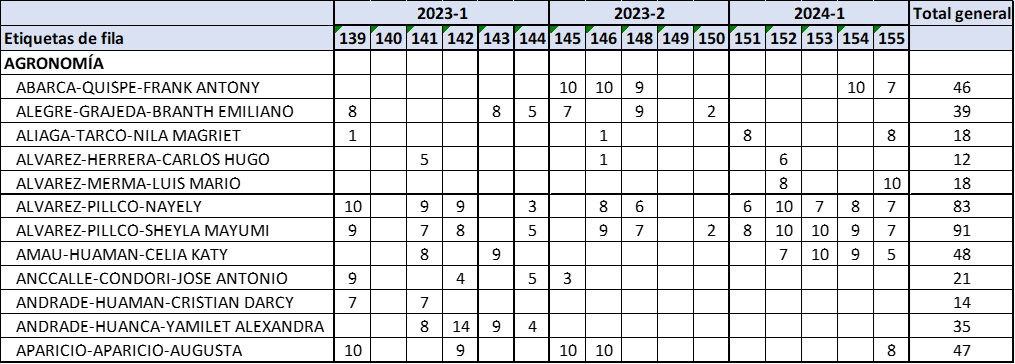
\includegraphics{imagen/cuadro1.png}

}

\end{figure}%

\subsection{Elaboración del registro de becados beneficiarios del
comedor universitario (2023-I, 2023-II y
2024-I)}\label{elaboraciuxf3n-del-registro-de-becados-beneficiarios-del-comedor-universitario-2023-i-2023-ii-y-2024-i}

En la segund aparte de la solicitud, se disponia elaborar un registro
para los becados beneficiarios del comedor, con el objetivo d
eidentificar a la población que hacia uso del beneficio y la que no mlo
hacia para establecer nuevos filtros en la selección de beneficiarios
del comedor universitario, para los cuales se tuvo las siguientes
características:

\begin{itemize}
\tightlist
\item
  Estudiantes organizados por escuela profesional
\item
  Veces en la que el estudiante ha hecho uso del comedor en un cupo
\end{itemize}

\begin{figure}[H]

\caption{Registro de becarios beneficiarios del comedor universitario
(2023-I, 2023-II y 2024-I)}

{\centering 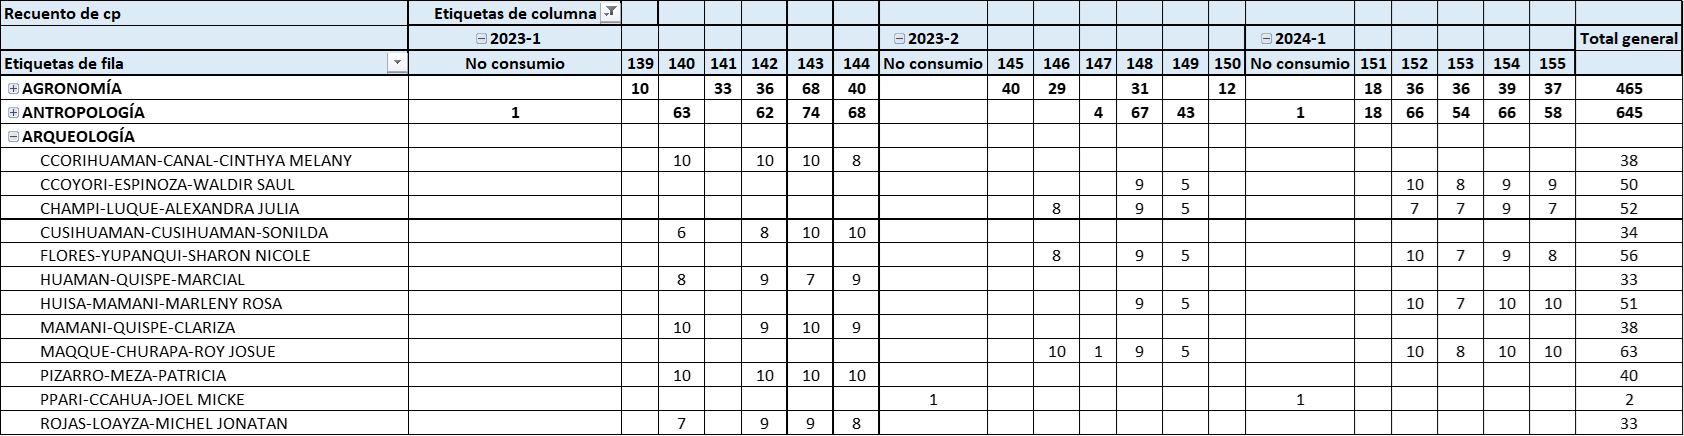
\includegraphics{imagen/cuadro2.png}

}

\end{figure}%

\subsection{Elaboración de estadísticos de los docentes nombrados en el
semestre
2024-1}\label{elaboraciuxf3n-de-estaduxedsticos-de-los-docentes-nombrados-en-el-semestre-2024-1}

\bookmarksetup{startatroot}

\chapter{Conclusiones}\label{conclusiones}

La realización de mis prácticas preprofesionales en la Oficina de
Gestión de la Calidad me permitió obtener una visión más profunda sobre
la situación actual de nuestra universidad y los procesos implementados
por el equipo de la oficina para mejorar cada aspecto y elevar la
calidad universitaria.

Este entorno me ayudó a expandir mis ideas y a considerar soluciones
fuera del contexto habitual para abordar problemas específicos. También
tuve la oportunidad de aplicar y desarrollar los conocimientos y
habilidades adquiridos durante mi formación universitaria.

Las actividades y procesos en los que participé fueron cruciales para el
avance de la Oficina de Gestión de la Calidad. Comprendí que los
procesos de calidad requieren un orden meticuloso y la ejecución
eficiente de tareas pequeñas para evitar deficiencias en las actividades
y asegurar la calidad general.

Todo proceso destinado a ser considerado de calidad debe seguir un orden
definido en su aplicación o desarrollo. Los procedimientos llevados a
cabo en la Universidad Nacional de San Antonio Abad del Cusco están
sujetos a un control riguroso, y los futuros procesos también deben
seguir un desarrollo bien estructurado. La próxima evaluación para la
renovación del Licenciamiento Institucional exigirá un proceso definido
que será supervisado por la Oficina de Gestión de la Calidad como
principal ente de verificación.

Aprendí mucho sobre el funcionamiento de la Oficina de Gestión de la
Calidad, la cual actúa como órgano asesor dentro de la UNSAAC,
gestionando y consolidando el sistema de gestión de calidad educativa.

También comprendí la importancia del trabajo en equipo. Mi experiencia
en la Oficina ha sido enriquecedora tanto a nivel profesional como
personal.

Agradezco a la Universidad Nacional de San Antonio Abad del Cusco por
brindarme la oportunidad de realizar mis prácticas en la Oficina de
Gestión de la Calidad, permitiéndome aplicar mis conocimientos en un
área específica. Expreso mi gratitud a las señoritas Milagros Echegaray
Mayorga, Yadira Ríos Caballero y Urzula del Carmen Fernández Palomino
por su apoyo y asistencia durante mi tiempo en la Oficina. Asimismo,
agradezco al Dr.~Walter Orestes Antezana Julián por la oportunidad de
realizar mis prácticas en esta entidad.

\bookmarksetup{startatroot}

\chapter{Recomendaciones}\label{recomendaciones}

Para los futuros practicantes, se aconseja que se integren de inmediato
al inicio de sus prácticas y se comprometan con cada tarea asignada o
seleccionada. Es crucial que se esfuercen al máximo y aprovechen al
máximo la experiencia para su desarrollo profesional.

Sugiero a los estudiantes que buscan realizar prácticas preprofesionales
considerar la Oficina de Gestión de la Calidad, ya que ofrece un entorno
que apoya y proporciona servicios valiosos para su formación. Asimismo,
es esencial que la Oficina continúe brindando un apoyo constante a los
estudiantes. Este respaldo fomenta un ambiente de confianza y
colaboración, facilitando así la culminación exitosa del proceso de
prácticas preprofesionales.

\bookmarksetup{startatroot}

\chapter{Asistencia}\label{asistencia}

\bookmarksetup{startatroot}

\chapter*{Referencias}\label{referencias}
\addcontentsline{toc}{chapter}{Referencias}

\markboth{Referencias}{Referencias}

\phantomsection\label{refs}
\begin{CSLReferences}{1}{0}
\bibitem[\citeproctext]{ref-fao}
Estadística, U. de. (2024). \emph{Unidad de Estadística - UNSAAC}.
\url{https://www.unsaac.edu.pe/unidad-de-estadistica-2/}

\end{CSLReferences}



\end{document}
